\section{Contexte \& Démarche}
\subsection{Contexte -- Equipe Intégration, Accompagnement Projet (transverse)}
Le project se déroule dans une équipe d'intégration. Le project est cadré par mon encadrant de stage qui désigne les objectifs du project. Pour le réaliser, je suis en accompagné d'un rérérent technique.

On a une organisation tranverse, le travail est autonomie, mais je le support de toute l'équipe.

\subsection{Démarche agile - devops}
Au sein de la VSCT, on met beaucoup de points sur la méthode agile et la discipiline "Devops"(lexique. \ref{lexi:devops}). Dans cet équipe, on applique un "Kanban"(lexique. \ref{lexi:kanban}) pour l'organisation des travaux.  Comme sur la figure (fig. \ref{fig:kanban}), chaque membre dispose d'une lighe sur le tableau et chaque ligne est découpé en trois parties: "TODO", "EN-COUR" et "DONE" qui correspondant aux tâches à faire, tâche en train de faire et tâches réalisés. Les esapces laissées à gauche sont pour des idées qu'on va pêut-être planifier un jour.

\begin{figure}[h]
\centering
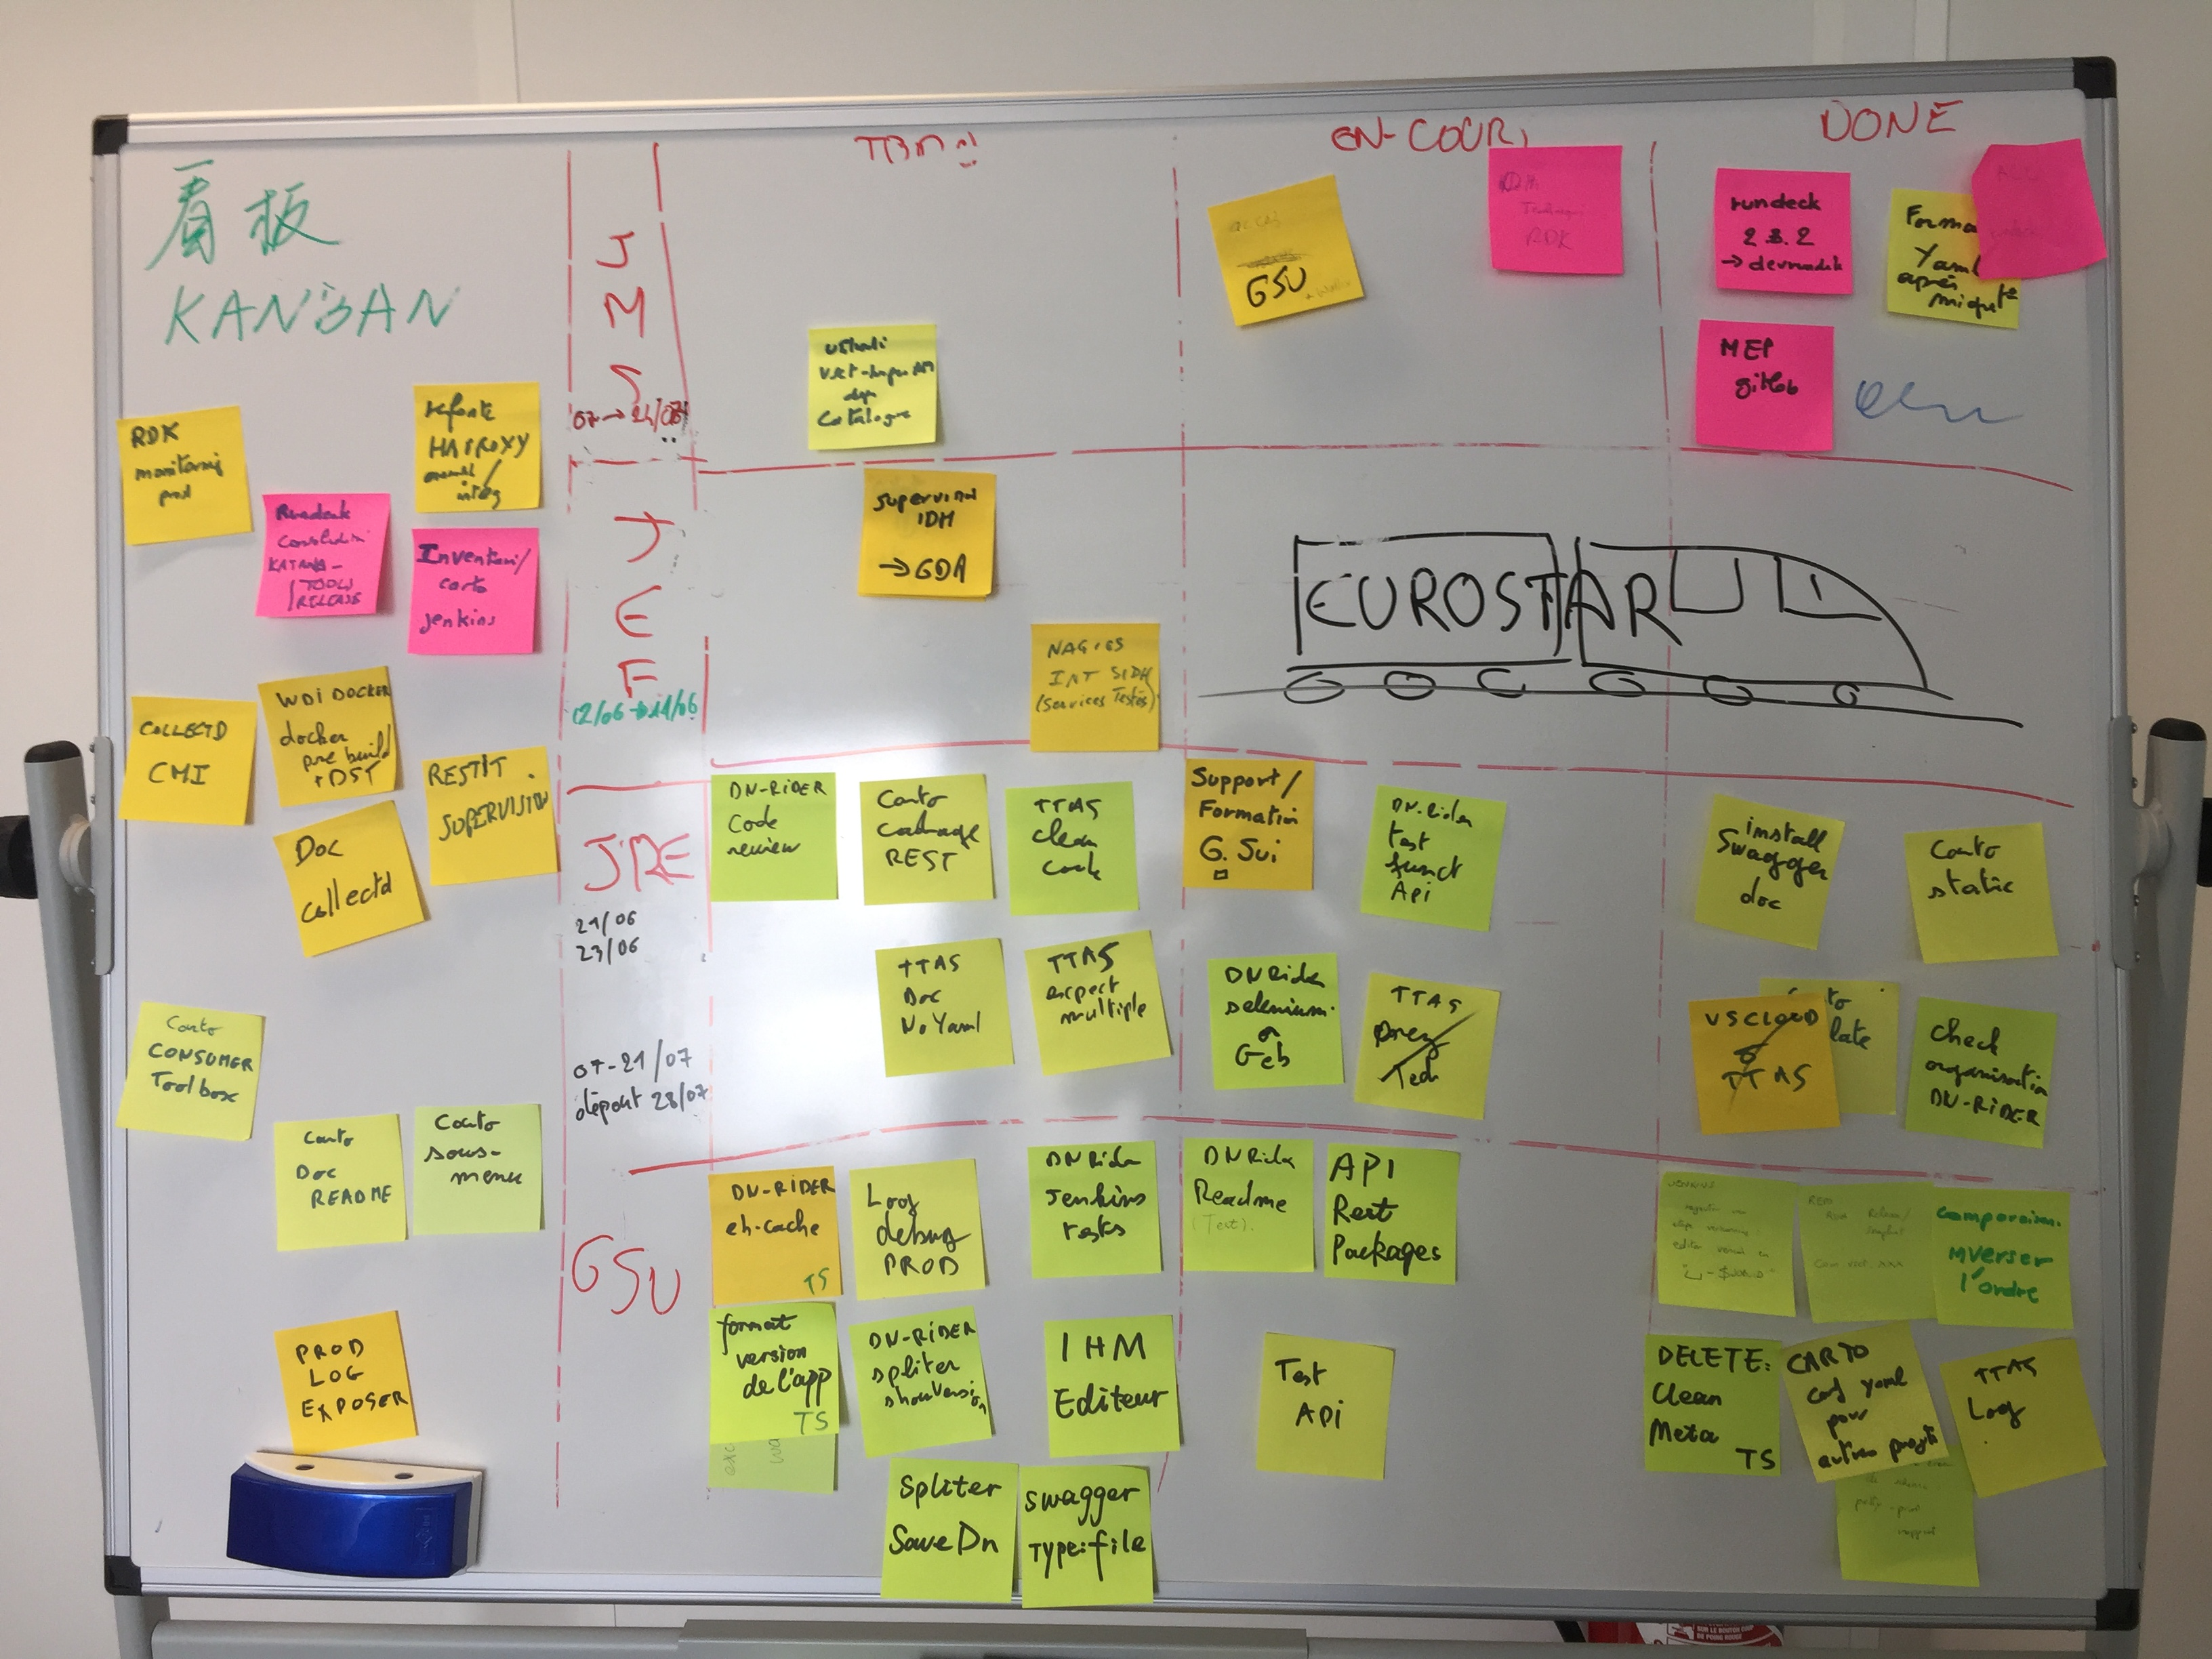
\includegraphics[width=0.8\textwidth]{kanban}
\caption{Kanban}
\label{fig:kanban}
\end{figure}

On applique la "post-it theory"(lexique. \ref{lexi:post_it_theory}). Les post-its sont classés par leur coleurs, les plus profonds correspondants aux tâches plus importants. Certains cartes sont marqué 'TS'(Technic Story) dessus, c'est-à-dire que c'est un petit sourcis technique qui est pas urgent à être résolu, on a une grande liberté de l'organiser seloon notre convenience.

Normalement on fait  deux fois par semine le review du Kanban pour garder le rythme. Chaque fois mes tuteurs valident ce que j'ai realisé et m'aident à planifier les tâches suivantes.

Les cods sources sont géré en git et stocké sur Gitlab. Au bout d'un mois et demi, on a la permière version de l'application et on commence à faire intégration continue en utilisant Jenkins pipeline. Chaque fois qu'il y a un commit sur la branche master, l'application seront déploié toutes seule.

\clearpage
